\section{Experimental Results \& Tests}
Using our implementation, TRE and scan\_for\_matches, we were able to do some benchmarking in order to compare performances.

Below is a table, with each of the files that our tests were executed on.\\

\begin{table}[h!]
\begin{tabular}{ c | c | c |  c | c | c | c |  c | c | c |  c }
 ~chr1.fa & ~chr2.fa  & ~chr3.fa & ~chr4.fa & ~chr5.fa & ~chr6.fa &  ~chr7.fa & ~chr8.fa & ~chr9.fa & chr10.fa & chr11.fa \\
 \hline
246.284 & 242.003 & 198.723 & 190.526 & 180.152 & 170.233 & 158.202 & 145.704 & 139.726 & 134.846 & 133.928
\end{tabular}
\begin{tabular}{ c | c | c |  c | c | c | c |  c | c | c |  c }
chr12.fa & chr13.fa & chr14.fa & chr15.fa & chr16.fa & chr17.fa & chr18.fa & chr19.fa & chr20.fa & chr21.fa & chr22.fa\\
\hline
131.833 & 113.698 & 105.954 & 99.947 & 88.481 & 78.468 & 75.820 & 63.563 & 62.193 & 46.761 & 49.498
\end{tabular}
\caption{Fasta files from http://hgdownload.cse.ucsc.edu/goldenPath/hg18/chromosomes/ with sizes in KB}
\label{tab:sizes}
\end{table}
Looking at Table~\ref{tab:sizes}, we have a series of fasta files, ranging from 246.284KB to 46.761 KB in size, each fasta file has a number, and besides $chr22.fa$, every number is decreasingly lower in size as to the previous.

Next we need to define a pattern upon which to test. As our implementation has primarily been focused on supporting insertion, deletion and mutation on a search pattern, a simple RNA sequence like $TGCAAGCGTTAAT$ will do fine.

We first ran a test using a single insertion in the pattern.
\begin{figure}[h!]
\centering
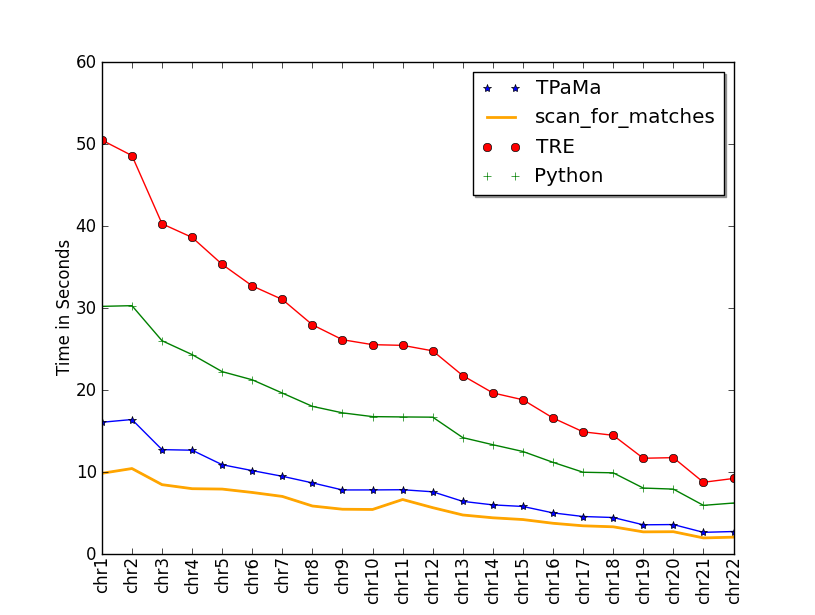
\includegraphics[width=0.6\textwidth]{Benchmarking/1ins.png}
\caption{Running time of search through fasta files mentioned in Table~\ref{tab:sizes},  allowing one insertions on pattern TGCAAGCGTTAAT}
\label{fig:ins1}
\end{figure}

(( NOTE: BENCHMARK WASNT COMPLETE AT TIME OF WRITING))
From Figure~\ref{fig:ins1}, it's clear that given the 22 files, scan\_for\_matches would always be faster, and our implementation would execute roughly at double the time. TRE however would be about 5 times slower than scan\_for\_matches on this simple pattern.
\newpage

Next we tested the same pattern, but with two insertions instead of one.
\begin{figure}[h!]
\centering
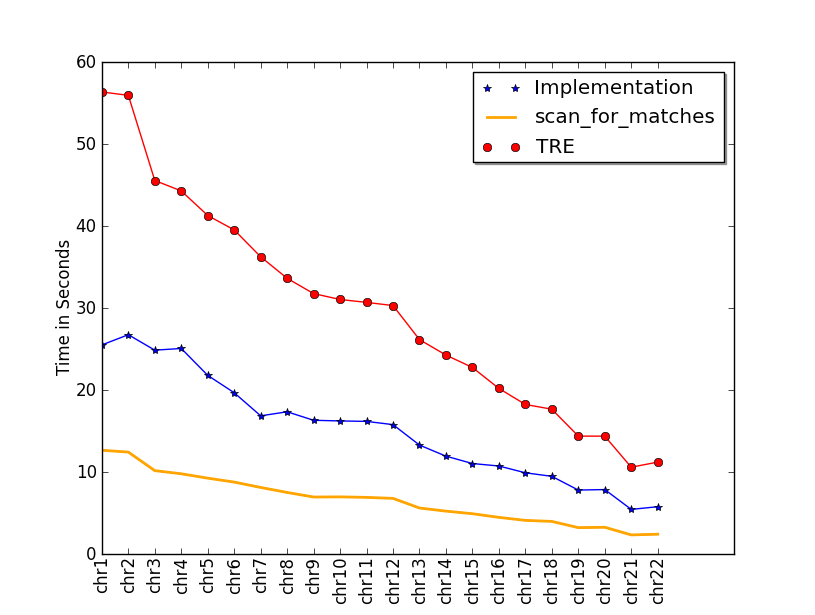
\includegraphics[width=0.6\textwidth]{Benchmarking/2ins.png}
\caption{Running time of search through fasta files mentioned in Table~\ref{tab:sizes},  allowing two insertions on pattern TGCAAGCGTTAAT}
\label{fig:ins2}
\end{figure}

While scan\_for\_matches did increase its runtime slightly, the second insertion really affected our implementation, resulting in it running at about the speed as TRE.  And while TRE also had its runtime slightly increased, it's almost unchanged from one insertion.

(( TODO: DISPLAY HITS ))